\chapter{Análisis de reactores reales}
\section{Funciones de Distribución de Edades}
\begin{flushleft}
    El comportamiento del flujo real en un sistema continuo se sitúa entre los dos límites ideales: el \textbf{Flujo en Pistón} (ausencia total de mezcla axial es decir $0\%$ de la mezcla) y la \textbf{Mezcla Perfecta} (mezcla instantánea y uniforme en todo el volumen es decir $100\%$ de la mezcla). Para caracterizar las desviaciones de la idealidad y cuantificar el grado de mezcla, se emplean las \textbf{Funciones de Danckwerts} o funciones de distribución de edades.

    Considerando un sistema de volumen $V$ atravesado por una corriente de caudal volumétrico $v_0$ (o $F$), definimos los elementos de fluido bajo las siguientes premisas fundamentales:
\end{flushleft}
\begin{itemize}
    \item \textbf{Identidad individual:} Los elementos son lo suficientemente pequeños para conservar su identidad durante su tránsito por el reactor (comportamiento de "paquete" de fluido).
    \item \textbf{Continuidad macroscópica:} Los elementos son lo suficientemente grandes para que las propiedades intensivas ($\rho, C_i, T$) estén bien definidas y sigan las leyes del continuo.
\end{itemize}



\dfn{Distribución de Edades y Tiempos de Residencia}{
    \begin{itemize}
        \item \textbf{Edad ($t$):} Tiempo transcurrido desde que un elemento entra al sistema.
        \item \textbf{Tiempo de residencia ($t_r$):} Edad de un elemento en el instante exacto en que abandona el sistema.

        \item \textbf{Distribución en el interior, $I(t)$:}
              \begin{equation*}
                  I(t) = \frac{\text{Fracción de elementos en el interior de edad } t}{\text{Unidad de tiempo}} \quad \rightarrow \quad I(t)\,dt
              \end{equation*}

        \item \textbf{Distribución en la salida, $E(t)$:}
              \begin{equation*}
                  E(t) = \frac{\text{Fracción de elementos en la salida de edad } t}{\text{Unidad de tiempo}} \quad \rightarrow \quad E(t)\,dt
              \end{equation*}
              \nt{La función $E(t)$ es la que define propiamente la \textbf{RTD} (\textit{Residence Time Distribution}).}
    \end{itemize}
}
\newpage
\noindent Ambas funciones lo que representan son las fracciones de elementos de unidad t en el sistema tal y como se ve en el siguiente esquema:

\begin{figure}[h]
    \begin{center}
        \begin{tikzpicture}[
                node distance=2.5cm,
                block/.style={rectangle, draw, fill=blue!10, thick, minimum width=3cm, minimum height=1.5cm, rounded corners},
                arrow/.style={->, >=stealth, ultra thick, blue!70!black},
                label_text/.style={font=\small\itshape, text width=4cm, align=center}
            ]

            % Nodo central (Sistema)
            \node (sistema) [block] {\textbf{SISTEMA}};

            % Flecha de entrada
            \draw [arrow] (-3,0) -- (sistema.west) node[midway, above, black] {$I(t)$};

            % Flecha de salida
            \draw [arrow] (sistema.east) -- (3,0) node[midway, above, black] {$E(t)$};

            % Explicaciones en la parte inferior
            \node (descI) [below left=of sistema, xshift=1cm, yshift=1cm, label_text] {
                $I(t)$: Fracción de elementos en el \textbf{interior} de edad $t$ por unidad de tiempo
            };

            \node (descE) [below right=of sistema, xshift=-1cm, yshift=1cm, label_text] {
                $E(t)$: Fracción de elementos en la \textbf{salida} de edad $t$ por unidad de tiempo
            };

            % Líneas opcionales para conectar leyenda con flechas
            \draw [dashed, gray] (-2.2,-0.2) -- (descI.north);
            \draw [dashed, gray] (2.2,-0.2) -- (descE.north);
        \end{tikzpicture}
        \caption{Funciones de distribución de edades}
        \label{fig:distribucion_edades}
    \end{center}
\end{figure}
\noindent si hacemos la integral de ambas funciones en un intervalo se ve mas claramente:
\begin{equation}
    \int_{t_1}^{t_2} I(t) dt = \text{Fracción de volumen del sistema de edad comprendida entre } t_1 \text{ y } t_2
\end{equation}
\begin{equation}
    \int_{t_1}^{t_2} E(t) dt = \text{Fracción de elementos en la salida de edad comprendida entre } t_1 \text{ y } t_2
\end{equation}
\noindent Y lo mismo ocurre si integramos en el tiempo total:
\begin{equation}
    \int_{0}^{\infty} I(t) dt = 1
\end{equation}
\begin{equation}
    \int_{0}^{\infty} E(t) dt = 1
\end{equation}
\nt{Es obvio que si hacemos la integral de la funcion $I(t)\,dt$, entre 0 y infinito todos los elementos estan en el interior del sistema, y por tanto como es una fracción la función I es decir un tanto por uno, la integral debe de valer uno. Por otro lado, si hacemos la integral de la funcion $E(t)\,dt$, entre 0 y infinito estamos calculando la fracción de todos los elementos que salen del sistema en todos los tiempos es decir todos los estaran en la corriente de salida, por tanto la integral de la funcion E(t) también vale uno}
\noindent Tambien es importante ver que cualquier magnitud que se promedie mediante la función $E(t)$lo que se esta calculando es su valor medio, es decir su valor ponderado y por tanto se puede hacer el siguiente calculo:
\begin{equation}
    t_R = \frac{V}{F} = \int_{0}^{\infty} t E(t) dt \text{ (tiempo de residencia)}
\end{equation}
\noindent Por otra parte si quisieramos que el tiempo fuera adimensional, lo que se haria seria:
\begin{equation}
    \theta = \frac{t}{t_R} \implies d\theta = I(\theta) = I(t)\cdot t_R , E(\theta) = E(t)\cdot t_R
\end{equation}
\noindent La relación entre ambas es evidente, una vez se han definido ambas funciones y teniendo claro lo que representan, pensando en el ejemplo de un sistema donde metemos unos elementos ese sistema esta en movimiento, y en un momento deben de salir del sistema, por tanto como se observa:

\begin{equation}
    \underbrace{E}_{\text{Edad salida}} = \underbrace{-\frac{dI}{d\theta}}_{\text{Variación edad interior}} \label{eq:defE}
\end{equation}
\nt{El signo negativo indica que la fracción de elementos con una determinada edad en el interior disminuye a medida que estos abandonan el sistema (pasan a la corriente de salida).}
\noindent Para obtener la relación acumulada, integramos la expresión diferencial considerando que en el instante inicial ($\theta = 0$), la fracción de elementos en el interior es la unidad ($I = 1$):

\begin{align*}
    \int_{1}^{I} dI          & = -\int_{0}^{\theta} E \, d\theta \quad \text{\scriptsize{Limite entre 1 y I}} \\[10pt]
    \left[ I \right]_{1}^{I} & = -\int_{0}^{\theta} E \, d\theta                                              \\[10pt]
    I - 1                    & = -\int_{0}^{\theta} E \, d\theta
\end{align*}

\noindent Reordenando los términos, obtenemos la expresión final que relaciona ambas funciones de distribución:

\begin{equation}
    I = 1 - \int_{0}^{\theta} E \, d\theta    \label{eq:defI}
\end{equation}
\section{Aplicación de las funciones E y I}
\subsection{Reactor continuo flujo de pistón}
\noindent entrarian a tiempo 0 iran avanzando a largo de todo el reactor y cuando el tiempo sea el de residencia esos elementos saldran del sistema, pero todos a la vez por tanto para cualquier tiempo inferior al tiempo de residencia todos los elementos estaran dentro del sistema y por tanto $I=1$, pero para cualquier tiempo superior al de residencia o dicho de forma $\theta>1$ no quedara ningun elemento dentro del sistema y por tanto $I=0$, esto matematicamente se conoce como la funcion en escalon unitario.
\begin{figure}[htbp]
    \centering
    % Parte superior: Ecuaciones y condiciones
    \begin{minipage}{0.4\textwidth}
        \begin{align*}
             & \text{Para } t \leq t_R \text{ ó } \theta \leq 1 \implies I = 1 \\
             & \text{Para } t > t_R \text{ ó } \theta > 1 \implies I = 0
        \end{align*}
    \end{minipage}
    \hfill
    % Parte derecha: Representación gráfica con TikZ (MÁS ANCHA)
    \begin{minipage}{0.55\textwidth}
        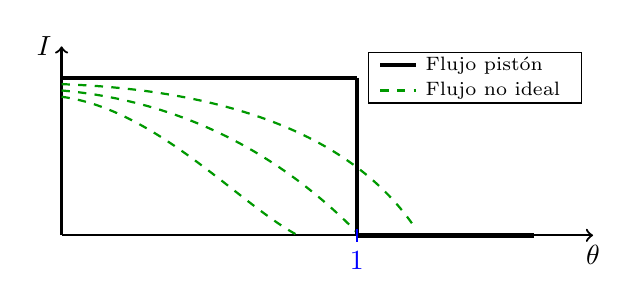
\begin{tikzpicture}[xscale=1.5, yscale=0.8] % Aumentado xscale para ensanchar
            % Ejes
            \draw[->, thick] (0,0) -- (4.5,0) node[below] {$\theta$};
            \draw[->, thick] (0,0) -- (0,3) node[left] {$I$};

            % Curvas de dispersión (líneas verdes discontinuas)
            \draw[green!60!black, thick, dashed] (0,2.4) .. controls (1.5,2.3) and (2.5,1.5) .. (3,0.1);
            \draw[green!60!black, thick, dashed] (0,2.3) .. controls (1.2,2.1) and (2.0,1.0) .. (2.5,0.05);
            \draw[green!60!black, thick, dashed] (0,2.2) .. controls (0.8,2.0) and (1.5,0.5) .. (2.0,0);

            % Función escalón ideal (Flujo Pistón)
            \draw[ultra thick] (0,2.5) -- (2.5,2.5); % El escalón ideal es una línea recta
            \draw[ultra thick] (2.5,2.5) -- (2.5,0); % Cae verticalmente en theta=1 (escalado a 2.5)
            \draw[ultra thick] (2.5,0) -- (4,0);

            % Etiqueta del 1 en el eje theta (escalado para coincidir con el escalón)
            \draw[blue, thick] (2.5,0.1) -- (2.5,-0.1) node[below] {$1$};

            % Leyenda manual
            \draw[fill=white, draw=black, thin] (2.6, 2.9) rectangle (4.4, 2.1);
            \draw[ultra thick] (2.7, 2.7) -- (3.0, 2.7);
            \node[right, font=\scriptsize] at (3.0, 2.7) {Flujo pistón};
            \draw[green!60!black, thick, dashed] (2.7, 2.3) -- (3.0, 2.3);
            \node[right, font=\scriptsize] at (3.0, 2.3) {Flujo no ideal};
        \end{tikzpicture}
    \end{minipage}

    \caption{Representación de la función de distribución interna para flujo ideal y desviaciones por dispersión.}
    \label{fig:distribucion_interna_escalon_ancha}
\end{figure}

\vspace{0.5cm}
\begin{flushleft}
    \textbf{Función en escalón unidad}
\end{flushleft}
\begin{equation}
    \begin{aligned}
        U(x - x_0) & = 0 \quad x < x_0 \\
        U(x - x_0) & = 1 \quad x > x_0
    \end{aligned}
    \hspace{2cm}
    \color{red} I = 1 - U(x - x_0)
\end{equation}
\noindent Donde tal y como se puede observar en la grafica anterior, se ve la idealización y aproximaciones del flujo pistón.
Si ahora lo hacemos para la función E tenemos lo siguiente:
\begin{figure}[htbp]
    \centering
    % Parte superior: Ecuaciones y condiciones para E
    \begin{minipage}{0.4\textwidth}
        \begin{align*}
             & \text{Para } t = t_R \text{ ó } \theta = 1 \implies E = \infty  \\
             & \text{Para } t \neq t_R \text{ ó } \theta \neq 1 \implies E = 0
        \end{align*}
    \end{minipage}
    \hfill
    % Parte derecha: Representación gráfica (Función Impulso y Dispersión)
    \begin{minipage}{0.55\textwidth}
        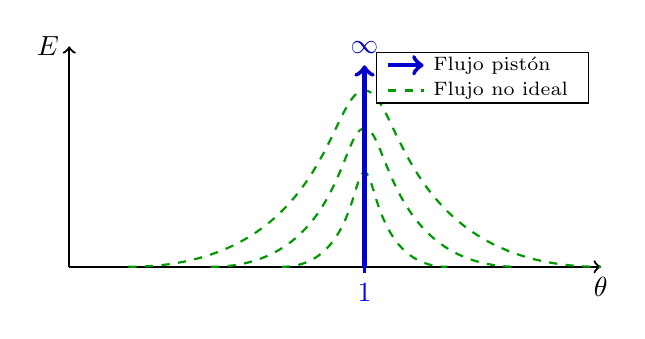
\begin{tikzpicture}[xscale=1.5, yscale=0.8]
            % Ejes
            \draw[->, thick] (0,0) -- (4.5,0) node[below] {$\theta$};
            \draw[->, thick] (0,0) -- (0,3.5) node[left] {$E$};

            % Curvas de dispersión (Campanas de Gauss - Líneas verdes discontinuas)
            % Representan el flujo real alejándose de la idealidad
            \draw[green!60!black, thick, dashed] (0.5,0) .. controls (2.2,0) and (2.2,2.8) .. (2.5,2.8) .. controls (2.8,2.8) and (2.8,0) .. (4.5,0);
            \draw[green!60!black, thick, dashed] (1.2,0) .. controls (2.3,0) and (2.3,2.2) .. (2.5,2.2) .. controls (2.7,2.2) and (2.7,0) .. (3.8,0);
            \draw[green!60!black, thick, dashed] (1.8,0) .. controls (2.4,0) and (2.4,1.5) .. (2.5,1.5) .. controls (2.6,1.5) and (2.6,0) .. (3.2,0);

            % Función Impulso ideal (Delta de Dirac - Flujo Pistón)
            \draw[ultra thick, blue!80!black, ->] (2.5,0) -- (2.5,3.2) node[above] {$\infty$};

            % Etiqueta del 1 en el eje theta
            \draw[blue, thick] (2.5,0.1) -- (2.5,-0.1) node[below] {$1$};

            % Leyenda manual
            \draw[fill=white, draw=black, thin] (2.6, 3.4) rectangle (4.4, 2.6);
            \draw[ultra thick, blue!80!black, ->] (2.7, 3.2) -- (3.0, 3.2);
            \node[right, font=\scriptsize] at (3.0, 3.2) {Flujo pistón};
            \draw[green!60!black, thick, dashed] (2.7, 2.8) -- (3.0, 2.8);
            \node[right, font=\scriptsize] at (3.0, 2.8) {Flujo no ideal};
        \end{tikzpicture}
    \end{minipage}

    \caption{Representación de la función de distribución de salida ($E$) para flujo pistón ideal (impulso) y sistemas con dispersión (curvas de campana).}
    \label{fig:distribucion_salida_impulso}
\end{figure}

\vspace{0.5cm}
\begin{flushleft}
    \textbf{Función impulso unidad o delta de Dirac}
\end{flushleft}
\begin{equation*}
    \begin{aligned}
        \delta(x - x_0) & = 0 \quad x \neq x_0   \\
        \delta(x - x_0) & = \infty \quad x = x_0
    \end{aligned}
    \hspace{2cm}
    \color{red} E = \delta(\theta - 1)
\end{equation*}


\nt{Como para cualquier t que sea el tiempo de residencia todos los elementos salen del sistema, y como todos salen en un instante, es decir, un punto, por eso la función E es infinito. Al ser en un instante (estaría dividido entre 0), el valor es $\infty$. Para cualquier otro tiempo $\theta \neq 1$, no quedará ningún elemento dentro del sistema y por tanto $E=0$.}
\noindent La función impulso se representa matemáticamente como la delta de Dirac, es decir:
\begin{equation}
    \begin{cases}
        \delta(x-x_0) = 0      & \quad x \neq x_0 \\
        \delta(x-x_0) = \infty & \quad x = x_0
    \end{cases}
    \hspace{2cm}
    \color{red} E = \delta(\theta - 1)
\end{equation}

\cor{Importante}{Representaciones de nuestros sistemas de la función E con un máximo en $\theta = 1$ nos indican que el reactor es de tipo ideal, es decir, flujo pistón. Los que estén próximos a ello serán reactores tubulares con comportamientos cercanos a la idealidad, es decir, al flujo pistón.}
\subsection{Reactor continuo mezcla perfecta (RCMP)}
\noindent En este reactor la mezcla es perfecta, es decir, hay una homogeneización completa en todo el sistema. Por tanto, la corriente de salida es idéntica a la del interior del reactor, por lo que la función E será idéntica a la I.
\begin{figure}[htbp]
    \centering

    %==================== PARTE IZQUIERDA ====================
    \begin{minipage}{0.4\textwidth}
        \begin{align}
            E                      & = I                                                                   \nonumber \\[6pt]
            E                      & = -\frac{dI}{d\theta} \implies I = -\frac{dI}{d\theta} \label{eq:E_I}           \\[8pt]
            d\theta                & = -\frac{dI}{I}                                                       \nonumber \\[8pt]
            \theta                 & = -\ln I                                                              \nonumber \\[6pt]
            \mathbf{\color{red} E} & \mathbf{\color{red} = I = \exp(-\theta)}
        \end{align}

    \end{minipage}
    \hfill
    %==================== GRAFICA ====================
    \begin{minipage}{0.55\textwidth}

        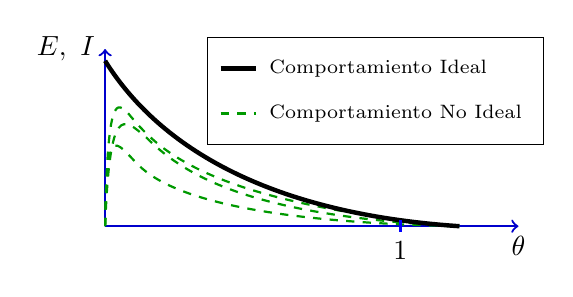
\begin{tikzpicture}[xscale=1.5,yscale=1.5]

            %---------------- EJES ----------------
            \draw[->, thick, blue!80!black]
            (0,0) -- (3.5,0)
            node[below, black] {$\theta$};

            \draw[->, thick, blue!80!black]
            (0,0) -- (0,1.5)
            node[left, black] {$E,\ I$};

            %---------------- CURVAS NO IDEALES ----------------
            % Ahora parten desde el origen

            \draw[green!60!black, dashed, thick]
            (0,0)
            .. controls (0.02,1.15) and (0.10,1.05)
            .. (0.20,0.95)
            .. controls (0.45,0.65) and (0.85,0.20)
            .. (3,0);

            \draw[green!60!black, dashed, thick]
            (0,0)
            .. controls (0.04,1.05) and (0.15,0.92)
            .. (0.35,0.75)
            .. controls (0.70,0.40) and (1.30,0.08)
            .. (3,0);

            \draw[green!60!black, dashed, thick]
            (0,0)
            .. controls (0.01,0.90) and (0.08,0.72)
            .. (0.28,0.52)
            .. controls (0.60,0.20) and (1.50,0.03)
            .. (3,0);

            %---------------- CURVA IDEAL ----------------
            \draw[ultra thick, black]
            (0,1.4)
            .. controls (0.5,0.6) and (1.5,0.1)
            .. (3,0);

            %---------------- MARCA theta = 1 ----------------
            \draw[blue, thick]
            (2.5,0.05) -- (2.5,-0.05);

            \node[below] at (2.5,-0.05) {$1$};

            %---------------- LEYENDA ----------------
            % Separada ligeramente para que no atraviesen el texto

            \matrix[
                draw,
                fill=white,
                font=\scriptsize,
                anchor=north east,
                row sep=2pt,
                inner sep=4pt
            ]
            at (3.72,1.6)
            {
                \draw[ultra thick, black]
                (0,0) -- (0.45,0);
                 &
                \node[anchor=west] {Comportamiento Ideal};
                \\

                \draw[green!60!black, thick, dashed]
                (0,0) -- (0.45,0);
                 &
                \node[anchor=west] {Comportamiento No Ideal};
                \\
            };

        \end{tikzpicture}

    \end{minipage}

    %==================== NOTA FUERA DE LA FIGURA ====================

    \caption{
        Distribución de edades en un RCMP. Comparación entre el comportamiento exponencial ideal y las desviaciones típicas representadas por las curvas no ideales.
    }

    \label{fig:RCMP_distribucion_final}

\end{figure}

%==================== NOTA EXTERNA ====================

\vspace{0.3cm}

\nt{En un reactor de mezcla perfecta ideal, la probabilidad de que un elemento de fluido salga ($E$) es exactamente igual a la fracción de elementos que aún permanecen en su interior ($I$).}
\section{Experimentos estímulo-respuesta}

\noindent En este apartado se estudia cómo determinar experimentalmente las funciones de distribución de edades ($E$ o $I$). El procedimiento estándar consiste en realizar experimentos de \textbf{estímulo-respuesta}, los cuales se basan en introducir una perturbación (trazador) en la entrada y analizar su evolución en la salida. Existen dos tipos principales:
\begin{itemize}
    \item Estimulo en \textbf{impulso} (inyección instantánea).
    \item Estimulo en \textbf{escalón} (inyección continua).
\end{itemize}

\subsection{Estímulo en escalón o estímulo continuo}

\begin{figure}[htbp]
    \centering
    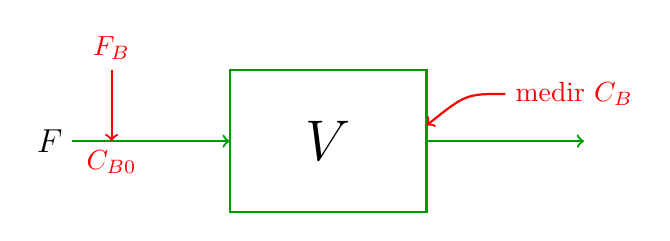
\begin{tikzpicture}[node distance=2cm, auto]
        % El Reactor (Caja verde)
        \draw[green!60!black, thick] (0,0) rectangle (2.5,1.8);
        \node at (1.25,0.9) {\huge $V$};

        % Corriente de entrada
        \draw[->, thick, green!60!black] (-2,0.9) -- (0,0.9);
        \node[anchor=east] at (-2,0.9) {\large $F$};
        \node[below, red] at (-1.5,0.9) {$C_{B0}$};

        % Inyección de trazador
        \draw[->, thick, red] (-1.5,1.8) node[above] {$F_B$} -- (-1.5,0.9);

        % Corriente de salida
        \draw[->, thick, green!60!black] (2.5,0.9) -- (4.5,0.9);

        % Indicador de medida
        \draw[<-, thick, red] (2.5,1.1) .. controls (3,1.5) .. (3.5,1.5) node[right] {medir $C_B$};
    \end{tikzpicture}
    \caption{Esquema de un experimento de estímulo en escalón.}
    \label{fig:experimento_estimulo_escalon}
\end{figure}
\begin{flushleft}
    En este experimento, se mantiene un caudal constante $F$ de disolvente a través de un reactor de volumen $V$. En un instante determinado ($t=0$), se introduce de forma continua una corriente de trazador $B$ (sustancia inerte y fácilmente medible, por ejemplo, mediante colorimetría o conductividad).

    Para no alterar la reología del sistema, el caudal del trazador ($F_B$) debe ser despreciable frente al caudal principal ($F_B \ll F$). La mezcla de ambas corrientes resulta en una concentración de entrada constante $C_{B0}$. A partir del inicio de la inyección, se monitoriza la concentración de salida $C_B(t)$ hasta que el sistema alcanza el estado estacionario, momento en el cual $C_B = C_{B0}$.

    A esta respuesta del sistema se le denomina \textbf{Función respuesta estímulo en escalón} ($F_{ee}$ o simplemente curva $F$), y se define de forma adimensional como:
\end{flushleft}
\begin{equation}
    \mathbf{F_{ee}(t) = \frac{C_B(t)}{C_{B0}}}
\end{equation}

\noindent Las condiciones experimentales que deben cumplirse son:
\begin{itemize}
    \item $F_B \ll F$ (Caudal de trazador despreciable).
    \item $C_{B0}$: Concentración constante del trazador en la alimentación para $t \ge 0$.
    \item $F_{ee} \in [0, 1]$ (Variable normalizada).
\end{itemize}

\noindent Los datos obtenidos se suelen tabular para su posterior tratamiento numérico:

\begin{table}[htbp]
    \centering
    \begin{tabular}{ccc}
        \hline
        \textbf{Tiempo ($t$)} & \textbf{Concentración ($C_{B}$)} & \textbf{Función $F_{ee}$} \\ \hline
        0                     & 0                                & 0                         \\
        $t_i$                 & $C_{B,i}$                        & $C_{B,i}/C_{B0}$          \\
        $\vdots$              & $\vdots$                         & $\vdots$                  \\
        $t_{\infty}$          & $C_{B0}$                         & 1                         \\ \hline
    \end{tabular}
    \caption{Datos experimentales de concentración y respuesta en escalón.}
    \label{tab:concentracion_tiempo}
\end{table}
\subsubsection{Balance al estado no estacionario}
\begin{alignat}{2}
     & \text{Balance: }                &  & \frac{d}{dt} \left( C_{B0} \cdot V \cdot \int_{0}^{t} I(t) \, dt \right) = F \cdot C_{B0} - F \cdot C_B \nonumber \\[10pt]
     & \text{Derivando la integral: }  &  & C_{B0} \cdot V \cdot I(t) = F \cdot C_{B0} - F \cdot C_B                                                \nonumber \\[10pt]
     & \text{Despejando } I(t):        &  & I(t) = \frac{F}{V} \frac{C_{B0}}{C_{B0}} - \frac{F}{V} \frac{C_B}{C_{B0}}                               \nonumber \\[10pt]
     & \text{Sustituyendo } t_R = V/F: &  & I(t) = \frac{1}{t_R} - \frac{1}{t_R} F_{EE}                                                             \nonumber \\[10pt]
     & \text{Resultado final: }        &  & \mathbf{\color{red} I = 1 - F_{EE}}
\end{alignat}
\noindent Ademas relacionando la función $E$ con la función $I$ tal y como se veia en ~\eqref{eq:E_I} tenemos que:
\begin{equation}
    E = -\frac{dI}{d\theta} = -\frac{dF_{EE}}{d\theta } \implies\boxed{E = \frac{dF_{EE}}{d\theta}}
\end{equation}
\subsection{Estímulo en impulso o estímulo instantáneo}
\begin{figure}[htbp]
    \centering
    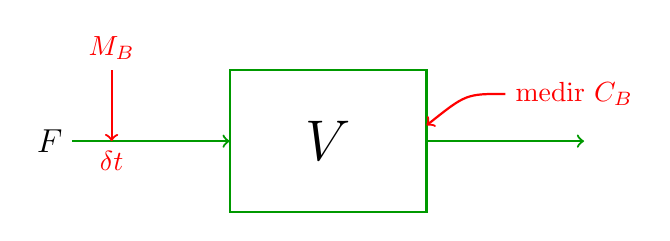
\begin{tikzpicture}[node distance=2cm, auto]
        % El Reactor (Caja verde)
        \draw[green!60!black, thick] (0,0) rectangle (2.5,1.8);
        \node at (1.25,0.9) {\huge $V$};

        % Corriente de entrada
        \draw[->, thick, green!60!black] (-2,0.9) -- (0,0.9);
        \node[anchor=east] at (-2,0.9) {\large $F$};
        \node[below, red] at (-1.5,0.9) {$\delta t$};

        % Inyección de trazador
        \draw[->, thick, red] (-1.5,1.8) node[above] {$M_B$} -- (-1.5,0.9);

        % Corriente de salida
        \draw[->, thick, green!60!black] (2.5,0.9) -- (4.5,0.9);

        % Indicador de medida
        \draw[<-, thick, red] (2.5,1.1) .. controls (3,1.5) .. (3.5,1.5) node[right] {medir $C_B$};
    \end{tikzpicture}
    \caption{Esquema de un experimento de estímulo en impulso.}
    \label{fig:experimento_estimulo_impulso}
\end{figure}
\begin{flushleft}
    En este experimento, se inyecta de forma instantánea una cantidad total de trazador $M_B$ (moles) en la entrada del reactor.\\
    La inyección debe ser lo suficientemente rápida como para que el trazador se distribuya uniformemente en el reactor antes de que comience el flujo. Es decir en un instante llamado $\delta t$.
    Posteriormente, se mide la concentración instantánea de trazador en la salida $C_B(t)$ a medida que este fluye fuera del reactor.\\

    A esta respuesta del sistema se le denomina \textbf{Función respuesta estímulo en impulso} ($I$, o simplemente curva $I$), y se define de forma adimensional como:
\end{flushleft}
\begin{equation}
    I(t) = \frac{C_B(t)}{C_{B0}} = \frac{C_B}{\dfrac{M_B}{V}}
\end{equation}
\noindent lo que ocurrira es que el tiempo partira en 0 hasta que se termine el estudio, la concentracion de B comenzara en 0, en un determinado momento llegara a su maximo y luego comenzara a disminuir hasta llegar a 0 ya que se ha metido un solo impulso es decir no es continuo, y la funcion respuesta
estimulo en impulso le ocurrira lo mismo. aunque ya se ha definido en la ecuacion anterior esta bien recordar que:
\dfn{}{
    \begin{multicols}{2}
        \begin{itemize}
            \item $C = \frac{C_B}{C_{BR}}$\\ es decir concentracion de B respecto a una concentracion de referencia.
            \item $C = \frac{C_B}{M_B/V}$\\ la concentración de referencia sera los moles que hemos metido $M_B$ respecto al volumen del reactor $V$.
        \end{itemize}
    \end{multicols}
}
\begin{table}[htbp]
    \centering
    \begin{tabular}{ccc}
        \hline
        \textbf{Tiempo ($t$)} & \textbf{Concentración ($C_{B}$)} & \textbf{C}  \\
        \hline
        0                     & 0                                & 0           \\
        $\vdots$              & $\vdots$                         & $\vdots$    \\
        $t_i$                 & $C_{B,max}$                      & $C_{i,max}$ \\
        $\vdots$              & $\vdots$                         & $\vdots$    \\
        $t_{\infty}$          & 0                                & 0           \\
        \hline
    \end{tabular}
    \caption{Datos experimentales de concentración y respuesta en impulso.}
    \label{tab:concentracion_tiempo_impulso}
\end{table}
\subsubsection{Balance al estado no estacionario}
\begin{alignat*}{3}
     & \text{Balance: }                         &  & \frac{d}{dt} \left( \underbrace{\frac{m_B}{F \cdot \textcolor{red}{\cancel{\Delta t}}}}_{\text{conc. de B}} \underbrace{ \cdot V \cdot I(t) \cdot \textcolor{red}{\cancel{\Delta t}} }_{\text{Volumen}} \right) = -F \cdot C_B &       &                                                                                                                \\[12pt]
     & \text{Agrupando } t_R:                   &  & \frac{d}{dt} \left( m_B \cdot \underbrace{\frac{V}{F}}_{t_R} \cdot I(t) \right) = -F \cdot C_B                                                                                                                                 &       &                                                                                                                \\[10pt]
     & \text{Cambio de } dt \text{ a } d\theta: &  & m_B \cdot \cancel{t_R} \cdot \frac{dI}{\cancel{t_R} \cdot d\theta} = -F \cdot C_B                                                                                                                                              & \quad & \textcolor{gray}{\leftarrow \text{usando } dt = t_R d\theta}                                                   \\[10pt]
     & \text{Normalizando: }                    &  & \underbrace{\frac{m_B}{ \textcolor{darkgreen}{F \cdot C_{BR}}}}_{t_R} \cdot \frac{dI}{d\theta} = -\frac{\cancel{F}\cdot C_B}{\cancel{F}\cdot C_{BR}}                                                                           & \quad & \textcolor{gray}{\leftarrow \text{recordando que: } C = C_B/C_{BR}}                                            \\[10pt]
     & \text{recordando que:}                   &  & \frac{m_B}                            {F\cdot \underbrace{m_B/V}_{C_{BR}}}      = \frac{V}{F} = t_R                                                                                                                            &       &                                                                                                                \\[10pt]
     & \text{Regla de la cadena: }              &  & t_R \cdot \left( \frac{dI}{d\theta} \cdot \textcolor{blue}{\frac{d\theta}{dt}} \right) = - \frac{C_B}{C_{BR}}\textcolor{gray}{\bigg]_C}                                                                                        &       &                                                                                                                \\[10pt]
     & \text{Sustituyendo diferencial: }        &  & \cancel{t_R} \cdot \frac{dI}{d\theta} \cdot \textcolor{blue}{\frac{1}{\cancel{t_R}}} = -C                                                                                                                                      & \quad & \textcolor{gray}{\leftarrow \text{ya que } \theta = \frac{t}{t_R} \implies \frac{d\theta}{dt} = \frac{1}{t_R}} \\[10pt]
     & \text{Relación final: }                  &  & -\frac{dI}{d\theta} = C = E \implies \mathbf{\color{red} E = C}                                                                                                                                                                & \quad & \implies    \boxed{I = 1 - \int_{0}^{\theta} C \, d\theta}                                                     \\[10pt]
\end{alignat*}
\nt{Se puede ver que E = C recordando la definición de E en la ecuación \eqref{eq:defE} y luego ver el resultado de la integral con la ecuación ~\eqref{eq:defI}.}
\subsection{Aplicación de la función E}
\noindent recordando que nuestra función E segun la delta de dirac para un reactor flujo pistón en $\theta$ = 1 salen todos los elementos tal y como se veia en la figura \ref{fig:distribucion_salida_impulso} y el caso contrario seria el mezcla perfecta. por tanto si aplicamos la varianza de la siguiente forma:
\begin{equation}
    \sigma^2 = \int_{0}^{\infty} \left( \theta - 1 \right)^2 E \, d\theta \label{eq:var_E}
\end{equation}
\noindent tendremos 2 casos:
\begin{itemize}
    \item Si \(\sigma^2 = 0\): el reactor es flujo pistón (todos los elementos salen al mismo tiempo).
    \item Si \(\sigma^2 > 0\): el reactor presenta dispersión (los elementos salen en diferentes momentos).
\end{itemize}
\noindent Si expandimos la ecuación ~\eqref{eq:var_E} y trabajamos un poco con ella obtendremos:
\begin{align*}
    \sigma^2 & = \int_{0}^{\infty} \left( \theta^2 - 2\theta + 1 \right) E \, d\theta                                                                                        \\
             & = \int_{0}^{\infty} \theta^2 E \, d\theta - \textcolor{darkgreen}{2 \int_{0}^{\infty} \theta E \, d\theta} + \textcolor{blue}{\int_{0}^{\infty} E \, d\theta} \\
             & = \int_{0}^{\infty} \theta^2 E \, d\theta - 1
\end{align*}
\nt{recordando que la E lo que hacia era promediar la variable que tenia delante, es decir la $\theta$ de forma que simplemente se resta el \textcolor{darkgreen}{-2} con el \textcolor{blue}{+1.}}

\begin{Definición}[colbacktitle=red!75!black]{Desviación del comportamiento de la idealidad}{}
En reactores reales, el patrón de flujo se aparta del modelo ideal. Esta desviación se cuantifica mediante la varianza adimensional:

\begin{center}
    \begin{minipage}{0.45\textwidth}
        \begin{equation}
            \color{red} \sigma^2 = \int_{0}^{\infty} \theta^2 E \, d\theta - 1
            \label{eq:varianza_adimensional}
        \end{equation}

    \end{minipage}
    \hfill
    \begin{minipage}{0.5\textwidth}
        \centering
        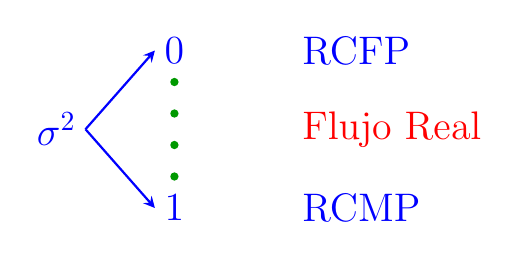
\begin{tikzpicture}[scale=1]
            % Nodos principales
            \node[blue, font=\Large] (sigma) at (0, 0) {$\sigma^2$};
            \node[blue, font=\Large] (cero) at (1.5, 1) {$0$};
            \node[blue, font=\Large] (uno)  at (1.5, -1) {$1$};

            % Flechas desde sigma
            \draw[-stealth, thick, blue] (sigma.east) -- (cero.west);
            \draw[-stealth, thick, blue] (sigma.east) -- (uno.west);

            % Puntos verdes intermedios
            \foreach \y in {0.6, 0.2, -0.2, -0.6} {
                    \fill[green!60!black] (1.5, \y) circle (1.5pt);
                }

            % Símbolos de implicación
            \node[blue, font=\Large] at (2.5, 1) {$\implies$};
            \node[blue, font=\Large] at (2.5, -1) {$\implies$};

            % Etiquetas finales
            \node[blue, font=\Large, anchor=west] at (3.0, 1) {RCFP};
            \node[red, font=\Large, anchor=west]  at (3.0, 0) {Flujo Real};
            \node[blue, font=\Large, anchor=west] at (3.0, -1) {RCMP};
        \end{tikzpicture}
    \end{minipage}
    \vspace{0.4cm}
    \small\textit{Clasificación del régimen de flujo en función de la varianza adimensional.}
\end{center}
\end{Definición}
\section{Modelización}
\begin{figure}[htbp]
    \centering
    \begin{tikzpicture}[xscale=1, yscale=1]
        % --- NIVEL 1: Varianza ---
        \node[font=\Large] (sigma) at (0, 0) {$\sigma^2$};

        % --- NIVEL 2: Valores 0 y 1 ---
        \node[myb, font=\Large] (cero) at (1.4, 1.0) {$\approx 0$};
        \node[myr, font=\Large] (uno)  at (1.4, -1.0) {$\approx 1$};

        % Flechas nivel 1
        \draw[-stealth, thick] (sigma.east) -- (cero.west);
        \draw[-stealth, thick] (sigma.east) -- (uno.west);

        % Símbolos de implicación
        \node[myb, font=\Large] at (2.3, 1.0) {$\implies$};
        \node[myr, font=\Large] at (2.3, -1.0) {$\implies$};

        % --- NIVEL 3: Tipos de Reactor ---
        \node[myb, font=\Large, anchor=west] (tubular) at (2.9, 1.0) {Reactor Tubular};
        \node[myr, font=\Large, anchor=west] (tanque)  at (2.9, -1.0) {Reactor Tanque Agitado};

        % --- NIVEL 4: Modelos (Ramificación del Tubular) ---
        \node[myb, font=\large, anchor=west] (disp)  at (9.0, 1.6) {Modelo de Dispersión};
        \node[myb, font=\large, anchor=west] (serie) at (9.0, 0.4) {Tanques en serie};

        \draw[-stealth, thick, myb] (tubular.east) -- (disp.west);
        \draw[-stealth, thick, myb] (tubular.east) -- (serie.west);

        % --- NIVEL 5: Modelos (Ramificación del Tanque) ---
        \node[myr, font=\large, anchor=west] (pfr_rec) at (9.0, -0.4) {PFR con recirculación};
        \node[myr, font=\large, anchor=west] (mezcl)   at (9.0, -1.6) {Tanques mezclados};

        \draw[-stealth, thick, myr] (tanque.east) -- (pfr_rec.west);
        \draw[-stealth, thick, myr] (tanque.east) -- (mezcl.west);

    \end{tikzpicture}
    \caption{Relación entre la varianza adimensional, el tipo de reactor y sus modelos matemáticos asociados.}
    \label{fig:modelizacion_sigma2_completo}
\end{figure}

\noindent De acuerdo con el grado de desviación de la idealidad (cuantificado por la varianza $\sigma^2$), se selecciona el modelo que mejor describa el patrón de flujo real del reactor:

\begin{itemize}
    \item \textbf{Reactores Tubulares:} Se modelan considerando una mezcla parcial. El modelo de \textit{tanques en serie} converge a un reactor de flujo pistón cuando el número de tanques $n \to \infty$; por tanto, un valor finito de $n$ describe la dispersión en un tubular. Alternativamente, se emplea el modelo de dispersión axial.
    \item \textbf{Reactores de Tanque Agitado:} Se suelen modelar mediante flujo pistón con recirculación o configuraciones de tanques mezclados para capturar cortocircuitos o zonas muertas.
\end{itemize}

\subsection{Ecuaciones de Modelización según la Varianza}

\begin{itemize}
    \item \textbf{Modelo de dispersión axial:}
          Se utiliza el número de dispersión ($N_D = D/uL$). Para recipientes abiertos:
          \begin{equation}
              \sigma^2_E = 2 N_D + 8 N_D^2
          \end{equation}
          O la expresión general (frecuentemente usada en recipientes cerrados):
          \begin{equation}
              \sigma^2_E = 2 N_D - 2 N_D^2 \left( 1 - \exp\left( -\frac{1}{N_D} \right) \right)
          \end{equation}

    \item \textbf{Modelo de tanques en serie:}
          Donde $n$ es el número de tanques ideales en serie:
          \begin{equation}
              \sigma^2_E = \frac{1}{n}
          \end{equation}

    \item \textbf{Modelo de flujo pistón con recirculación:}
          Relaciona la varianza con la relación de recirculación $R$:
          \begin{equation}
              \sigma^2_E = \frac{R}{(1+R)}
          \end{equation}

    \item \textbf{Diagnóstico de No Idealidades (Tanques mezclados):}
          Permite identificar fallos en el diseño hidrodinámico:
          \begin{itemize}
              \item \textbf{Presencia de \textit{Bypass} (Cortocircuito):}
                    Si el área bajo la curva es menor a la unidad:
                    \begin{equation}
                        \int_{0}^{\infty} E \, d\theta = 1 - X_{\text{bypass}}
                    \end{equation}
                    El porcentaje de elementos que no entran al reactor (\% \textit{bypass}) es $1 - \int_{0}^{\infty} E \, d\theta$.

              \item \textbf{Volumen Estancado (Zonas muertas):}
                    Se identifica mediante el primer momento de la curva:
                    \begin{equation}
                        \int_{0}^{\infty} \theta E \, d\theta = \frac{V_{activo}}{V_{total}}
                    \end{equation}
                    Si el resultado es menor que 1, el volumen estancado es $1 - \int_{0}^{\infty} \theta E \, d\theta$ (expresado en \%).
          \end{itemize}

    \item \textbf{Modelo de flujo segregado:} \label{sec:flujo_segregado}
          Aplicable exclusivamente a sistemas lineales (cinéticas de primer orden). Permite predecir la conversión media promediando la concentración individual de los 'paquetes' de fluido según su tiempo de residencia y si comparamos su resultado con el resto de modelos dara un resultado similar al mas optimo posible:
          \begin{equation}
              \overline{C_A} = \int_{0}^{\infty} C_A(\theta) \cdot E(t) \, d\theta \label{eq:flujo_segregado_1}
          \end{equation}
          Este modelo proporciona el límite de rendimiento para sistemas con segregación completa.
\end{itemize}
\nt{En el caso de tener un volumen estancado, siempre debemos usar el modelo de diagnóstico de no idealidades (tanques mezclados). Aunque si la cinética es de primer orden también se podría usar el modelo de flujo segregado, ya que debería coincidir la conversión, es preferible el primer método debido a que nos permite calcular el porcentaje de \textit{bypass} y de volumen estancado.}
\section{Modelo de flujo segregado}
\noindent Para cinéticas de primer orden, partimos de la definición de la variación de concentración de $A$ respecto al tiempo:

\begin{alignat}{3}
     & \text{Ley de velocidad:}                    &  & \frac{dC_A}{dt} = -k \cdot C_A                                      &       & \nonumber                                                        \\[10pt]
     & \text{Separación de variables:\hspace{2em}} &  & \frac{dC_A}{C_A} = -k \cdot dt                                      &       & \nonumber                                                        \\[10pt]
     & \text{Integración:}                         &  & \int_{C_{A0}}^{C_{AS}} \frac{dC_A}{C_A} = -k \int_{0}^{t} dt        &       & \nonumber                                                        \\[10pt]
     & \text{Resolución:}                          &  & \ln\left(\frac{C_{AS}}{C_{A0}}\right) = -k \cdot t                  &       & \nonumber                                                        \\[10pt]
     & \text{Forma exponencial:}                   &  & C_{AS} = C_{A0} \cdot e^{-k \cdot t}                                &       & \nonumber                                                        \\[10pt]
     & \text{Cambio a } \theta:                    &  & \mathbf{C_A(\theta) = C_{A0} \cdot \exp(-k \cdot t_R \cdot \theta)} & \quad & \textcolor{gray}{\leftarrow \text{usando } t = t_R \cdot \theta} \\[10pt] \label{eq:flujo_segregado_concentracion}
\end{alignat}
\noindent Sustituyendo \eqref{eq:flujo_segregado_1} en la ecuación de mezcla de flujos, se obtiene:

\begin{equation}
    \overline{C_A} = \int_{0}^{\infty} C_{A0} \cdot e^{-k \cdot t_R \cdot \theta} \cdot E(t) \, d\theta
\end{equation}
\noindent Recordando que la función $E(\theta)$ actúa como un operador de promedio para la propiedad que la acompaña, y partiendo de la definición de conversión:

\begin{equation}
    C_A(\theta) = C_{A0}(1-X_A(\theta)) \quad \text{y} \quad \overline{C_{As}} = C_{A0}(1-\overline{X_{As}})
\end{equation}

\noindent Sustituyendo en la ecuación del modelo de flujo segregado:

\begin{equation}
    \cancel{C_{A0}}(1-\overline{X_{As}}) = \int_{0}^{\infty} \cancel{C_{A0}} (1-X_A(\theta)) \cdot E(\theta) \, d\theta
\end{equation}

\noindent De forma análoga si hacemos los mismos pasos para la conversión:
\begin{alignat}{3}
     & \text{Relación de conversión:}              &  & C_A = C_{A0}(1 - X_A)                                              & \quad & \nonumber                                                                                             \\[10pt]
     & \text{Derivada de la ley:}                  &  & \cancel{C_{A0}} \frac{dX_A}{dt} = k \cdot \cancel{C_{A0}}(1 - X_A) & \quad & \textcolor{gray}{\leftarrow \frac{dC_A}{dt} = -C_{A0} \frac{dX_A}{dt}} \nonumber                      \\[10pt]
     & \text{Separación de variables:\hspace{2em}} &  & \frac{dX_A}{1 - X_A} = k \cdot dt                                  & \quad & \nonumber                                                                                             \\[10pt]
     & \text{Integración:}                         &  & \int \frac{dX_A}{1 - X_A} = \int k \cdot dt                        & \quad & \nonumber                                                                                             \\[10pt]
     & \text{Resolución (Logaritmos):}             &  & -\ln(1 - X_A) = k \cdot t                                          & \quad & \nonumber                                                                                             \\[10pt]
     & \text{Forma exponencial:}                   &  & (1 - X_A) = \exp(-k \cdot t)                                       & \quad & \nonumber                                                                                             \\[10pt]
     & \text{Cambio a } \theta:                    &  & \mathbf{1 - X_A(\theta) = \exp(-k \cdot t_R \cdot \theta)}         & \quad & \textcolor{gray}{\leftarrow \text{usando } t = t_R \cdot \theta}     \label{eq:flujo_segregado_final} \\[10pt]
\end{alignat}
\section{Ejemplos practicos}
\subsection{Experimento en Escalón}

\noindent normalmente nos daran el tiempo y la concentración, aunque no nos diran si es el ensayo en estimulo o en escalón se puede observar que la concentración llega a un valor estacionario y por tanto es un ensayo en escalón.
\begin{table}[htbp]
    \centering
    \caption{Datos y cálculos del Experimento en Escalón.}
    \label{tab:excel_escalon_nuevo}
    \resizebox{\textwidth}{!}{
        \begin{tabular}{cccccccccccc}
            \toprule
            \textbf{$t$}                        & \textbf{$C_B$} & \textbf{$\theta$} & \textbf{$F_{ee}$} & \textbf{$1-F_{ee}$} & \textbf{$\theta_{medio}$} & \textbf{$E$} & \textbf{$\theta\cdot E$} & \textbf{$\theta^2\cdot E$} & \textbf{$\int E \, d\theta$} & \textbf{$\int \theta E \, d\theta$} & \textbf{$\int \theta^2 E \, d\theta$} \\
            (min)                               & (mM)           &                   &                   &                     &                           &              &                          &                            &                              &                                     &                                       \\ \midrule
            0                                   & 0              & 0                 & 0                 & 1                   & 0                         & 0.3          & 0                        & 0                          & -                            & -                                   & -                                     \\
            2                                   & 3              & 0.2               & 0.06              & 0.94                & 0.1                       & 0.3          & 0.03                     & 0.003                      & 0.03                         & 0.0015                              & 0.00015                               \\
            4                                   & 6              & 0.4               & 0.12              & 0.88                & 0.3                       & 0.3          & 0.09                     & 0.027                      & 0.06                         & 0.012                               & 0.003                                 \\
            6                                   & 9              & 0.6               & 0.18              & 0.82                & 0.5                       & 0.3          & 0.15                     & 0.075                      & 0.06                         & 0.024                               & 0.0102                                \\
            8                                   & 11             & 0.8               & 0.22              & 0.78                & 0.7                       & 0.2          & 0.14                     & 0.098                      & 0.05                         & 0.029                               & 0.0173                                \\
            \rowcolor{blue!20} 10               & 16             & 1                 & 0.32              & 0.68                & 0.9                       & 0.5          & 0.45                     & 0.405                      & 0.07                         & 0.059                               & 0.0503                                \\
            \rowcolor{red!20} 12                & 32             & 1.2               & 0.64              & 0.36                & 1.1                       & 1.6          & 1.76                     & 1.936                      & 0.21                         & 0.221                               & 0.2341                                \\
            14                                  & 49             & 1.4               & 0.98              & 0.02                & 1.3                       & 1.7          & 2.21                     & 2.873                      & 0.33                         & 0.397                               & 0.4809                                \\
            16                                  & 50             & 1.6               & 1                 & 0                   & 1.5                       & 0.1          & 0.15                     & 0.225                      & 0.18                         & 0.236                               & 0.3098                                \\
            18                                  & 50             & 1.8               & 1                 & 0                   & 1.7                       & 0            & 0                        & 0                          & 0.01                         & 0.015                               & 0.0225                                \\
            20                                  & 50             & 2                 & 1                 & 0                   & 1.9                       & 0            & 0                        & 0                          & 0                            & 0                                   & 0                                     \\ \midrule
            \rowcolor{green!15} \textbf{$\sum$} &                &                   &                   &                     &                           &              &                          &                            & \textbf{1}                   & \textbf{0.9945}                     & \textbf{1.12825}                      \\ \bottomrule
        \end{tabular}
    }
\end{table}

\begin{figure}[htbp]
    \centering
    \begin{minipage}{0.4\textwidth}
        \centering
        \begin{tabular}{|c|c|}
            \hline
            \rowcolor{orange!20} \textbf{$V$}  & 40 \, \si{L}        \\ \hline
            \rowcolor{orange!20} \textbf{$F$}  & 4 \, \si{L/min}     \\ \hline
            \rowcolor{orange!20} \textbf{$FB$} & 0.2 \, \si{mol/min} \\ \hline
        \end{tabular}
        \caption{Datos dados por el enunciado del problema.}
        \vspace{0.5cm}
        \begin{tabular}{|c|c|c|}
            \hline
            \rowcolor{orange!20} \textbf{$t_R$}    & \multicolumn{2}{c|}{10}                  \\ \hline
            \rowcolor{orange!20} \textbf{$C_{B0}$} & 0.05 \si{mol/L}         & 50 \si{mMol/L} \\ \hline
        \end{tabular}
        \vspace{0.2cm}
        \caption{Parámetros del experimento.}
        \vspace{0.3cm}
        \textbf{Nota:} $t_R = V/F$, $C_{B0} = F_{B}/F$
    \end{minipage}
    \hfill
    \begin{minipage}{0.55\textwidth}
        \centering
        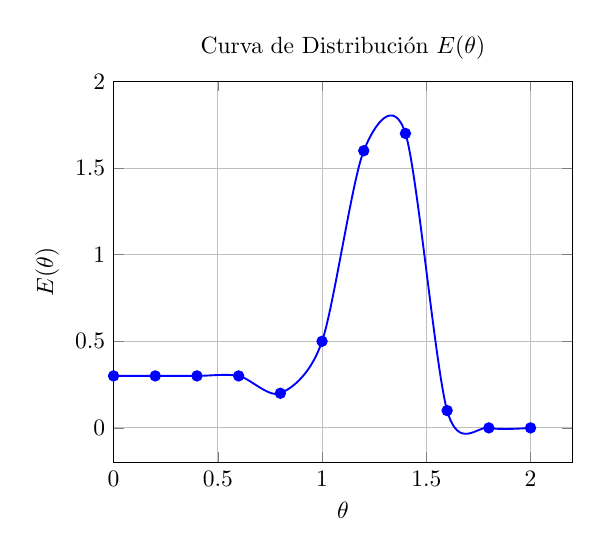
\begin{tikzpicture}[scale=0.85]
            \begin{axis}[
                    xlabel={$\theta$},
                    ylabel={$E(\theta)$},
                    grid=major,
                    xmin=0, xmax=2.2,
                    ymin=-0.2, ymax=2,
                    title={Curva de Distribución $E(\theta)$}
                ]
                \addplot[thick, blue,smooth, mark=*] coordinates {
                        (0,0.3)(0.2,0.3)(0.4,0.3)(0.6,0.3)(0.8,0.2)(1,0.5)(1.2,1.6)(1.4,1.7)(1.6,0.1)(1.8,0)(2,0)
                    };
            \end{axis}
        \end{tikzpicture}
    \end{minipage}
    \caption{Distribución de tiempos de residencia $E(\theta)$ obtenida a partir del escalón.}
\end{figure}
\newpage
\nt{El dato de $E$ para $t=0$ ($E_0 = 0.3$) puede no suministrarse en el enunciado original. Sin embargo, analizando la tendencia del resto de los datos experimentales, se deduce que el experimento comienza efectivamente en ese valor, procediéndose a realizar la corrección necesaria.}
\noindent lo primero que hacemos es dividir \textbf{$t/t_R$} y \textbf{$C_B/C_{B0}$} para obtener $\theta$ y $F_{EE}$ la funcion $E$ se obtiene como $E=dF_{EE}/d\theta$ de forma que se sigue el siguiente orden:
\begin{enumerate}
    \item Calcular el tiempo de residencia $t_R = V/F$

    \item Obtener el tiempo adimensional $\theta = t/t_R$

    \item Calcular la concentración inicial de B:
          $C_{B0} = F_{B}/F$

    \item Calcular la función de respuesta al estímulo escalón:
          \textbf{$F_{EE} = C_{B}/C_{B0}$}

    \item Calcular la función de distribución:
          \textbf{$E = dF_{EE}/d\theta$}

    \item Calcular $\theta \cdot E$ y $\theta^2 \cdot E$

    \item Calcular las integrales mediante el método de los trapecios
          (o trapecios acumulados para obtener directamente el sumatorio, que es lo que interesa)
\end{enumerate}
\noindent Procedemos a calcular un ejemplo:
\ex{Las filas seleccionadas corresponden a las resaltadas en \textcolor{blue}{azul} y \textcolor{red}{rojo}:}{
    \begin{enumerate}
        \item \textbf{Tiempo de residencia:} $t_R = V/F = 40/4 = 10 \si{min}$
        \item \textbf{Tiempo adimensional:} $\theta = t/t_R \implies \theta_{blue} = \textcolor{blue}{\frac{10}{10}=1}$ y $\theta_{red} = \textcolor{red}{\frac{12}{10}=1.2}$
        \item \textbf{Concentración inicial de B:} $C_{B0} = F_{B}/F = \frac{0.2}{4} = 0.05 \si{mol/L} = 50 \si{mMol/L}$
        \item \textbf{Respuesta al escalón:} $F_{EE} = C_{B}/C_{B0} \implies \textcolor{blue}{\frac{16}{50}=0.32}$ \quad y \quad $\textcolor{red}{\frac{32}{50}=0.64}$
        \item \textbf{Función de distribución:} $E = \frac{dF_{EE}}{d\theta} = \frac{\textcolor{red}{0.64} - \textcolor{blue}{0.32}}{\textcolor{red}{1.2} - \textcolor{blue}{1}} = 1.6$ (para $t=12$).
        \item \textbf{Cálculo de momentos:} Se usa el $\theta_{\text{medio}}$.
              Resultados: $\textcolor{blue}{0.5,\ 0.45,\ 0.405}$ y $\textcolor{red}{1.6,\ 1.76,\ 1.936}$
        \item \textbf{Integrales por trapecios:}
              \begin{itemize}
                  \item $\int E \, d\theta = \frac{(\textcolor{red}{1.6}+\textcolor{blue}{0.5})}{2} \cdot (\textcolor{red}{1.1}-\textcolor{blue}{0.9}) = \textcolor{red}{0.21}$
                  \item $\int \theta E \, d\theta = \frac{(\textcolor{red}{1.76}+\textcolor{blue}{0.45})}{2} \cdot (\textcolor{red}{1.1}-\textcolor{blue}{0.9}) = \textcolor{red}{0.221}$
                  \item $\int \theta^2 E \, d\theta = \frac{(\textcolor{red}{1.936}+\textcolor{blue}{0.405})}{2} \cdot (\textcolor{red}{1.1}-\textcolor{blue}{0.9}) = \textcolor{red}{0.2341}$
              \end{itemize}
        \item \textbf{Sumatorias finales:} Consultar la Tabla \ref{tab:excel_escalon_nuevo}.
    \end{enumerate}
}
\subsubsection{Modelización}
\noindent Aunque por la forma de la gráfica se identifica un reactor tubular, el análisis de los momentos confirma el diagnóstico:

\begin{alignat*}{2}
     & \text{Área total:}           &  & \int_{0}^{\infty} E \, d\theta = 1.00                                                                   \\
     & \text{Primer momento:} \quad &  & \int_{0}^{\infty} \theta E \, d\theta = 0.9945 \approx 1
    \quad \textcolor{gray}{(\text{Error } < 5\%, \text{ sin volumen muerto})}                                                                    \\
     & \text{Varianza:}             &  & \sigma^2 = \int_{0}^{\infty} \theta^2 E \, d\theta - 1 = 1.12825 - 1 = 0.12825                          \\
     & \text{Conclusión:}           &  & \sigma^2 \in (0; 0.5)\quad \xLongrightarrow{\hspace{1.4cm}} \boxed{\text{Reactor Tubular (Flujo Real)}}
\end{alignat*}
\section*{Deducción de la Conversión Acumulada (Orden 1)}

\noindent Partimos del balance de materia para el componente $A$ en el tanque $i$-ésimo de una batería de $n$ tanques en serie de igual volumen:

\begin{equation}
    k \cdot \tau_i = \frac{X_{Ai} - X_{A,i-1}}{1 - X_{Ai}}
\end{equation}

\subsection*{1. Despeje de la conversión de salida ($X_{Ai}$)}

Multiplicamos en cruz para eliminar el denominador:
\begin{equation}
    k \tau_i (1 - X_{Ai}) = X_{Ai} - X_{A,i-1}
\end{equation}

Agrupamos los términos que contienen $X_{Ai}$ en el lado derecho:
\begin{equation}
    k \tau_i + X_{A,i-1} = X_{Ai} + k \tau_i X_{Ai} \implies k \tau_i + X_{A,i-1} = X_{Ai}(1 + k \tau_i)
\end{equation}

Despejamos $X_{Ai}$:
\begin{equation}
    X_{Ai} = \frac{k \tau_i + X_{A,i-1}}{1 + k \tau_i}
\end{equation}

\subsection*{2. Transformación a la fracción no reaccionada ($1 - X_{Ai}$)}

Para encontrar la forma recursiva, restamos ambos lados de la unidad:
\begin{equation}
    1 - X_{Ai} = 1 - \frac{k \tau_i + X_{A,i-1}}{1 + k \tau_i} = \frac{(1 + k \tau_i) - (k \tau_i + X_{A,i-1})}{1 + k \tau_i}
\end{equation}

Simplificando los términos $k \tau_i$:
\begin{equation}
    1 - X_{Ai} = \frac{1 - X_{A,i-1}}{1 + k \tau_i}
\end{equation}

\subsection*{3. Aplicación de la serie para $n$ tanques}

\noindent Como la relación se repite para cada tanque desde $i=1$ hasta $n$, y sabiendo que a la entrada del primer tanque la conversión es nula ($X_{A0} = 0$):

\begin{itemize}
    \item \textbf{Tanque 1:} $(1 - X_{A1}) = \frac{1}{1 + k \tau_i}$
    \item \textbf{Tanque 2:} $(1 - X_{A2}) = \frac{1 - X_{A1}}{1 + k \tau_i} = \frac{1}{(1 + k \tau_i)^2}$
    \item \textbf{Tanque $n$:} $(1 - X_{An}) = \frac{1}{(1 + k \tau_i)^n}$
\end{itemize}

\subsection*{4. Expresión Final}

\noindent Aplicando la resolución en cascada para una batería de $n=8$ tanques suponiendo $k\tau_i = 0.25$ al no disponer del dato:
\begin{alignat*}{2}
     & \text{Conversión tras el tanque 7:} \quad &  & X_{A7} = 1 - \frac{1}{(1 + 0.25)^7} = \mathbf{0.7903} \\
     & \text{Conversión tras el tanque 8:}       &  & X_{AS} = 1 - \frac{1}{(1 + 0.25)^8} = \mathbf{0.8323}
\end{alignat*}

\noindent El salto de conversión en el último tanque es:
\begin{equation}
    \Delta X_A = X_{A8} - X_{A7} = 0.8323 - 0.7903 = 0.042 \implies \mathbf{4.2\%}
\end{equation}

\newpage
\subsection{Experimento de Impulso}

\nt{En este caso es conocido el tiempo y la concentración de B, pero se desconoce tanto el caudal como el volumen como el número de moles que se meten en la inyección del impulso}

\begin{table}[htbp]
    \centering
    \caption{Datos y cálculos del Experimento de Impulso.}
    \label{tab:excel_impulso_nuevo}
    \resizebox{\textwidth}{!}{
        \begin{tabular}{cccccccccccc}
            \toprule
            \textbf{$t$}                        & \textbf{$C_B$} & \textbf{$t\cdot C_B$} & \textbf{$\int t C_B \, dt$} & \textbf{$\int C_B \, dt$} & \textbf{$\theta$} & \textbf{$E$} & \textbf{$\theta\cdot E$} & \textbf{$\theta^2\cdot E$} & \textbf{$\int E \, d\theta$} & \textbf{$\int \theta E \, d\theta$} & \textbf{$\int \theta^2 E \, d\theta$} \\
            (min)                               & (mg/L)         &                       &                             &                           &                   &              &                          &                            &                              &                                     &                                       \\ \midrule
            0                                   & 0              & 0                     & -                           & -                         & 0                 & 0            & 0                        & 0                          & -                            & -                                   & -                                     \\
            1                                   & 9              & 9                     & 4.5                         & 4.5                       & 0.066             & 0.085        & 0.006                    & 0.000                      & 0.003                        & 0.000                               & 0.000                                 \\
            2                                   & 57             & 114                   & 61.5                        & 33                        & 0.132             & 0.540        & 0.071                    & 0.009                      & 0.021                        & 0.003                               & 0.000                                 \\
            3                                   & 81             & 243                   & 178.5                       & 69                        & 0.198             & 0.767        & 0.152                    & 0.030                      & 0.043                        & 0.007                               & 0.001                                 \\
            4                                   & 90             & 360                   & 301.5                       & 85.5                      & 0.264             & 0.853        & 0.225                    & 0.059                      & 0.053                        & 0.012                               & 0.003                                 \\
            5                                   & 90             & 450                   & 405                         & 90                        & 0.330             & 0.853        & 0.281                    & 0.093                      & 0.056                        & 0.017                               & 0.005                                 \\
            6                                   & 86             & 516                   & 483                         & 88                        & 0.396             & 0.815        & 0.322                    & 0.128                      & 0.055                        & 0.020                               & 0.007                                 \\
            8                                   & 77             & 616                   & 1132                        & 163                       & 0.528             & 0.729        & 0.385                    & 0.203                      & 0.102                        & 0.047                               & 0.022                                 \\
            10                                  & 67             & 670                   & 1286                        & 144                       & 0.660             & 0.635        & 0.419                    & 0.276                      & 0.090                        & 0.053                               & 0.032                                 \\
            \rowcolor{blue!20} 15               & 47             & 705                   & 3437.5                      & 285                       & 0.989             & 0.445        & 0.440                    & 0.436                      & 0.178                        & 0.142                               & 0.117                                 \\
            \rowcolor{red!20} 20                & 32             & 640                   & 3362.5                      & 197.5                     & 1.319             & 0.303        & 0.400                    & 0.528                      & 0.123                        & 0.139                               & 0.159                                 \\
            30                                  & 15             & 450                   & 5450                        & 235                       & 1.979             & 0.142        & 0.281                    & 0.556                      & 0.147                        & 0.225                               & 0.357                                 \\
            41                                  & 7              & 287                   & 4053.5                      & 121                       & 2.704             & 0.066        & 0.179                    & 0.485                      & 0.076                        & 0.167                               & 0.378                                 \\
            52                                  & 3              & 156                   & 2436.5                      & 55                        & 3.430             & 0.028        & 0.097                    & 0.334                      & 0.034                        & 0.100                               & 0.297                                 \\
            67                                  & 1              & 67                    & 1672.5                      & 30                        & 4.419             & 0.009        & 0.042                    & 0.185                      & 0.019                        & 0.069                               & 0.257                                 \\ \midrule
            \rowcolor{green!15} \textbf{$\sum$} &                &                       & \textbf{24264.5}            & \textbf{1600.5}           &                   &              &                          &                            & \textbf{1}                   & \textbf{1}                          & \textbf{1.636}                        \\ \bottomrule
        \end{tabular}
    }
\end{table}

\begin{figure}[htbp]
    \centering
    \begin{minipage}{0.4\textwidth}
        \centering
        \begin{tabular}{|c|c|}
            \hline
            \rowcolor{orange!20} \textbf{$t_R$}    & 15.161  \\ \hline
            \rowcolor{orange!20} \textbf{$C_{BR}$} & 105.570 \\ \hline
        \end{tabular}

        \vspace{0.5cm}
        \begin{tabular}{|c|c|}
            \hline
            \rowcolor{orange!20} \textbf{$\sigma^2$} & 0.636 \\ \hline
            \rowcolor{orange!20} \textbf{$R$}        & 1.747 \\ \hline
        \end{tabular}
        \vspace{0.2cm}
        \caption{Parámetros del experimento.}
    \end{minipage}
    \hfill
    \begin{minipage}{0.55\textwidth}
        \centering
        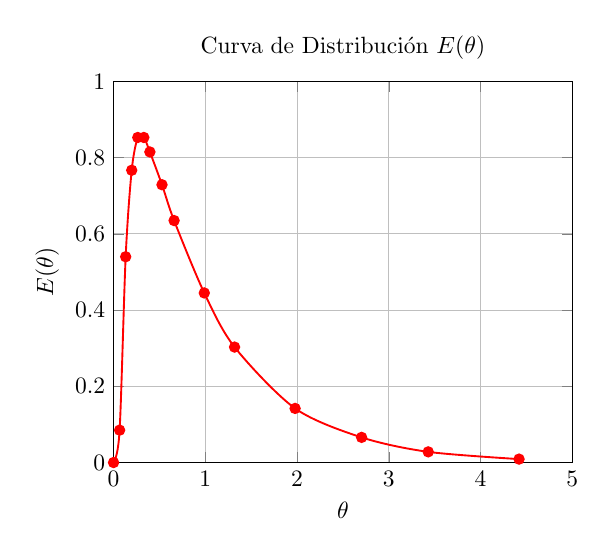
\begin{tikzpicture}[scale=0.85]
            \begin{axis}[
                    xlabel={$\theta$},
                    ylabel={$E(\theta)$},
                    grid=major,
                    xmin=0, xmax=5,
                    ymin=0, ymax=1,
                    title={Curva de Distribución $E(\theta)$}
                ]
                \addplot[thick, red, smooth, mark=*] coordinates {
                        (0,0)(0.066,0.085)(0.132,0.54)(0.198,0.767)(0.264,0.853)(0.33,0.853)(0.396,0.815)(0.528,0.729)(0.66,0.635)(0.989,0.445)(1.319,0.303)(1.979,0.142)(2.704,0.066)(3.43,0.028)(4.42,0.009)
                    };
            \end{axis}
        \end{tikzpicture}
    \end{minipage}
    \caption{Distribución de tiempos de residencia $E(\theta)$ obtenida a partir del impulso.}
\end{figure}
\nt{Aunque se aclara que es el experimento en impulso, se puede observar clarammente que partimos desde una concentración $C_B = 0$ y volvemos a dicho valor}
\begin{alignat*}{2}
     & \text{Normalización:}          &  & \int_{0}^{\infty} E \, d\theta = 1 \xLongrightarrow{\hspace{1cm}} \textcolor{gray}{\int_{0}^{\infty} C \, d\theta = 1}                                       \\[10pt]
     & \text{Sustituyendo } E:        &  & \int_{0}^{\infty} \frac{C_B}{C_{BR}} \, d\theta = 1 \xLongrightarrow{\hspace{1cm}} \textcolor{gray}{\int_{0}^{\infty} \frac{C_B}{m_B/V} d\theta = 1}         \\[10pt]
     & \text{Reordenando:}            &  & \int_{0}^{\infty} C_B \, d\theta = \frac{m_B}{F} \xLongrightarrow{\hspace{1cm}} \textcolor{gray}{C_{BR} = \frac{m_B}{V}}                                     \\[18pt]
     & \text{Primer momento:}         &  & \int_{0}^{\infty} \theta E \, d\theta = 1 \xLongrightarrow{\hspace{1cm}} \textcolor{gray}{\int_{0}^{\infty} \theta C \, d\theta = 1}                         \\[10pt]
     & \text{Sustituyendo variables:} &  & \int_{0}^{\infty} \frac{t}{t_R} \cdot \frac{C_B}{C_{BR}} \cdot \frac{dt}{t_R} = 1 \xLongrightarrow{\hspace{1cm}} \textcolor{gray}{\theta = \frac{t}{t_R}}    \\[10pt]
     & \text{Agrupando términos:}     &  & \int_{0}^{\infty} t C_B dt = t_R^2 C_{BR} \xLongrightarrow{\hspace{1cm}} \textcolor{gray}{t_R^2 \frac{m_B}{V}}                                               \\[10pt]
     & \text{Usando } t_R = V/F:      &  & \int_{0}^{\infty} t C_B dt = \frac{V^2}{F^2} \frac{m_B}{V} = \frac{m_B V}{F^2}                                                                               \\[18pt]
     & \text{Finalmente:}             &  & \boxed{t_R = \frac{\int_{0}^{\infty} t C_B dt}{\int_{0}^{\infty} C_B dt}} \xLongrightarrow{\hspace{1cm}} \textcolor{gray}{\text{Tiempo medio de residencia}} \\[15pt]
     & \text{Además:}                 &  & \boxed{C_{BR} = \frac{m_B/V}{F/V} = \frac{\int_{0}^{\infty} C_B dt}{t_R}}
\end{alignat*}
\ex{Las filas seleccionadas corresponden a las resaltadas en \textcolor{blue}{azul} y \textcolor{red}{rojo}:}{
    \begin{enumerate}
        \item \textbf{Tiempo de residencia:} $= \frac{\sum \int t C_B \, dt }{\sum \int C_B \, dt}=  24264.5/1600.5 = 15.161 \si{min}$
        \item \textbf{Tiempo adimensional:} $\theta = t/t_R \implies \theta_{blue} = \textcolor{blue}{\frac{15}{15.161}=0.989}$ y $\theta_{red} = \textcolor{red}{\frac{20}{15.161}=1.319}$
        \item \textbf{Concentración inicial de B:} $\frac{\sum \int C_B \,dt}{t_R} = \frac{1600.5}{15.161} = 105.570 \si{mMol/L}$
        \item \textbf{Función de distribución:} $E = \frac{C_B}{C_{BR}} = \textcolor{red}{\frac{32}{105.57}}=0.303 \quad y \quad \textcolor{blue}{\frac{47}{105.57}}=0.445$
        \item \textbf{Cálculo de momentos:} Se usa el $\theta_{\text{medio}}$.
              Resultados: $\textcolor{blue}{0.445,\ 0.440,\ 0.436}$ y $\textcolor{red}{0.303,\ 0.400,\ 0.528}$
        \item \textbf{Integrales por trapecios:}
              \begin{itemize}
                  \item $\int E \, d\theta = \frac{(\textcolor{red}{0.303}+\textcolor{blue}{0.445})}{2} \cdot (\textcolor{red}{1.319}-\textcolor{blue}{0.989}) = \textcolor{red}{0.173}$
                  \item $\int \theta E \, d\theta = \frac{(\textcolor{red}{0.400}+\textcolor{blue}{0.440})}{2} \cdot (\textcolor{red}{1.319}-\textcolor{blue}{0.989}) = \textcolor{red}{0.221}$
                  \item $\int \theta^2 E \, d\theta = \frac{(\textcolor{red}{0.528}+\textcolor{blue}{0.436})}{2} \cdot (\textcolor{red}{1.319}-\textcolor{blue}{0.989}) = \textcolor{red}{0.2341}$
              \end{itemize}
        \item \textbf{Sumatorias finales:} Consultar la Tabla \ref{tab:excel_impulso_nuevo}.
    \end{enumerate}
}
\subsubsection{Modelización}
\begin{alignat*}{2}
     & \text{Área total:}           &  & \int_{0}^{\infty} E \, d\theta = 1.00                                                                  \\
     & \text{Primer momento:} \quad &  & \int_{0}^{\infty} \theta E \, d\theta = 1                                                              \\
     & \text{Varianza:}             &  & \sigma^2 = \int_{0}^{\infty} \theta^2 E \, d\theta - 1 = 1.636 - 1 = 0.636                             \\
     & \text{Conclusión:}           &  & \sigma^2 \in (0.5; 1)\quad \xLongrightarrow{\hspace{1.4cm}} \boxed{\text{Reactor tipo tanque agitado}}
\end{alignat*}
\noindent la forma mas correcta de resolverlo, es mediante la modelización del reactor flujo pistón con recirculación, ya que agrega cierto grado de mezcla, y el de los tanques mezclados, al no tener un volumen estanco, no tiene sentido aplicarlo.
\begin{equation}
    \sigma^2 = \frac{R}{1+R} \implies R = 1.747
\end{equation}
\begin{equation}
    \tau = (1+R) \cdot C_{AR} \int_{X_{Ae}}^{X_{As}} \frac{d_{XA}}{r_A} \implies \tau = (1+R) \int_{\dfrac{X_{AR}}{R+1}}^{X_{As}} \frac{d_{XA}}{k\cdot (1-X_A)}
\end{equation}

\noindent tal y como se explicaba en la ecuación \ref{eq:RCFP_recirculacion_tau} de la sección \ref{sec:RCFP_Recirculacion_final} y recordando que el valor de R se obtiene de la siguiente manera:
\begin{equation}
    \sigma^2 = \frac{R}{1+R} \implies 0.636 = \frac{R}{1+R} \implies R = 1.7465
\end{equation}
\noindent Además el valor de k es de 0.304 min$^{-1}$, y la conversión de entrada es de 0 por lo que resolviendo\\

\begin{center}
    \Res{
        \tau = (1+R) \int_{\dfrac{X_{AR}}{R+1}}^{X_{As}} \frac{d_{XA}}{k\cdot (1-X_A)} \implies X_{As} = 0.905
    }
\end{center}
\nt{Al ser una cinética de primer orden también se puede hacer la modelización por flujo segregado repasando la sección \ref{sec:flujo_segregado} y finalmente en la ecuación \ref{eq:flujo_segregado_final} }


\ex{De forma análoga al caso anterior}{
    \small
    \begin{multicols}{3}
        \textbf{1.} Columna (\textbf{$1-X(\theta)$}) (Ec. \ref{eq:flujo_segregado_final}):
        \begin{itemize}
            \item $\exp(-0.304 \cdot 15.161 \cdot \textcolor{blue}{0}) = 1$
            \item $\exp(-0.304 \cdot 15.161 \cdot \textcolor{red}{0.066}) = 0.7379$
            \item $\exp(-0.304 \cdot 15.161 \cdot \textcolor{darkgreen}{0.132}) = 0.5444$
        \end{itemize}
        \columnbreak
        \textbf{2.} Columna (\textbf{$1-X(\theta)\cdot E$}):
        \begin{itemize}
            \item $\textcolor{blue}{1} \cdot \textcolor{blue}{0} = 0$
            \item $\textcolor{red}{0.7379} \cdot \textcolor{red}{0.085} = 0.0629$
            \item $\textcolor{darkgreen}{0.5444} \cdot \textcolor{darkgreen}{0.540} = 0.2940$
        \end{itemize}
        \columnbreak
        \textbf{3.} Integral (Trapecios):
        \begin{itemize}
            \item Para $\theta=0 \implies 0$
            \item $\frac{\textcolor{red}{0.0629}+\textcolor{blue}{0}}{2} \cdot (\textcolor{red}{0.066}-\textcolor{blue}{0}) = \textcolor{red}{0.0021}$
            \item $\left(\frac{\textcolor{darkgreen}{0.2940}+\textcolor{red}{0.0629}}{2} \cdot (\textcolor{darkgreen}{0.132}-\textcolor{red}{0.066})\right) + \textcolor{red}{0.0021} = \textcolor{darkgreen}{0.0138}$
        \end{itemize}
    \end{multicols}
    \vspace{0.2cm}
    \normalsize
    \textbf{4.} El último valor de la integral corresponde a la fracción no reaccionada a la salida ($1-X_A$).
}
\begin{table}[htbp]
    \centering
    \caption{Datos y cálculos para el modelo de flujo segregado.}
    \label{tab:flujo_segregado}
    \begin{tabular}{cccccc}
        \toprule
        \textbf{$t$ (min)}    & \textbf{$\theta$} & \textbf{$E$} & \textbf{$1-X(\theta)$} & \textbf{$(1-X)\cdot E$} & \textbf{$1-X$ media} \\ \midrule
        \rowcolor{blue!20} 0  & 0                 & 0            & 1.0000                 & 0.0000                  & 0                    \\
        \rowcolor{red!20} 1   & 0.066             & 0.085        & 0.7379                 & 0.0629                  & 0.0021               \\
        \rowcolor{green!20} 2 & 0.132             & 0.540        & 0.5444                 & 0.2940                  & 0.0138               \\
        3                     & 0.198             & 0.767        & 0.4017                 & 0.3082                  & 0.0337               \\
        4                     & 0.264             & 0.853        & 0.2964                 & 0.2527                  & 0.0522               \\
        5                     & 0.330             & 0.853        & 0.2187                 & 0.1865                  & 0.0667               \\
        6                     & 0.396             & 0.815        & 0.1614                 & 0.1315                  & 0.0772               \\
        8                     & 0.528             & 0.729        & 0.0879                 & 0.0641                  & 0.0901               \\
        10                    & 0.660             & 0.635        & 0.0478                 & 0.0304                  & 0.0963               \\
        15                    & 0.989             & 0.445        & 0.0105                 & 0.0047                  & 0.1021               \\
        20                    & 1.319             & 0.303        & 0.0023                 & 0.0007                  & 0.1030               \\
        30                    & 1.979             & 0.142        & 0.0001                 & 0.0000                  & 0.1032               \\
        41                    & 2.704             & 0.066        & 0.0000                 & 0.0000                  & 0.1032               \\
        52                    & 3.430             & 0.028        & 0.0000                 & 0.0000                  & 0.1032               \\
        67                    & 4.419             & 0.009        & 0.0000                 & 0.0000                  & 0.1032               \\ \bottomrule
    \end{tabular}
\end{table}
\begin{center}
    \Res{
        1-X_A(\theta) = \exp(-k \cdot t_R \cdot \theta) \implies X_A = 0.8968 \approx 0.90
    }
\end{center}
\noindent Aunque los datos puedan parecer más favorables en el modelo de flujo de pistón con recirculación que en el modelo de flujo segregado, en realidad este último es el más riguroso y adecuado. Es importante recalcar que ambos modelos deben coincidir al tratarse de una cinética de primer orden; la ligera variación en el resultado se debe únicamente a errores de redondeo en los cálculos numéricos.

\newpage
\subsection{Modelos Mezclados}


\begin{table}[htbp]
    \centering
    \small
    \caption{Cálculos detallados para ejemplo de modelos mezclados}
    \label{tab:excel_escalon}
    \begin{tabular}{ccccccc}
        \toprule
        \textbf{$t$}                        & \textbf{$C_B$} & \textbf{$\theta$} & \textbf{$E(\theta)$} & \textbf{$\theta\cdot E$} & \textbf{$\int E \, d\theta$} & \textbf{$\int E\cdot\theta \, d\theta$} \\
        (min)                               & (mg/L)         & ($t/t_R$)         & -                    & -                        & (Normalizado)                & (Momento)                               \\ \midrule
        0                                   & -              & 0                 & 1                    & 0                        & -                            & -                                       \\
        20                                  & 0.1            & 0.2083            & 0.8                  & 0.1667                   & 0.1875                       & 0.0174                                  \\
        40                                  & 0.079          & 0.4167            & 0.632                & 0.2633                   & 0.1492                       & 0.0448                                  \\
        60                                  & 0.063          & 0.625             & 0.504                & 0.315                    & 0.1183                       & 0.0602                                  \\
        80                                  & 0.05           & 0.8333            & 0.4                  & 0.3333                   & 0.0942                       & 0.0675                                  \\
        100                                 & 0.039          & 1.0417            & 0.312                & 0.325                    & 0.0742                       & 0.0686                                  \\
        \rowcolor{blue!20} 120              & 0.031          & 1.25              & 0.248                & 0.31                     & 0.0583                       & 0.0661                                  \\
        \rowcolor{red!20} 140               & 0.025          & 1.4583            & 0.2                  & 0.2917                   & 0.0467                       & 0.0627                                  \\
        160                                 & 0.019          & 1.6667            & 0.152                & 0.2533                   & 0.0367                       & 0.0568                                  \\
        180                                 & 0.015          & 1.875             & 0.12                 & 0.225                    & 0.0283                       & 0.0498                                  \\
        200                                 & 0.012          & 2.0833            & 0.096                & 0.2                      & 0.0225                       & 0.0443                                  \\
        228                                 & 0.01           & 2.375             & 0.08                 & 0.19                     & 0.0257                       & 0.0569                                  \\
        240                                 & 0.008          & 2.5               & 0.064                & 0.16                     & 0.0090                       & 0.0219                                  \\
        260                                 & 0.006          & 2.7083            & 0.048                & 0.13                     & 0.0117                       & 0.0302                                  \\
        280                                 & 0.005          & 2.9167            & 0.04                 & 0.1167                   & 0.0092                       & 0.0257                                  \\
        300                                 & 0.004          & 3.125             & 0.032                & 0.1                      & 0.0075                       & 0.0226                                  \\
        360                                 & 0.002          & 3.75              & 0.016                & 0.06                     & 0.0150                       & 0.0500                                  \\
        420                                 & 0.001          & 4.375             & 0.008                & 0.035                    & 0.0075                       & 0.0297                                  \\
        480                                 & 0.0005         & 5                 & 0.004                & 0.02                     & 0.0038                       & 0.0172                                  \\ \midrule
        \rowcolor{green!15} \textbf{$\sum$} &                &                   &                      &                          & \textbf{0.9051}              & \textbf{0.7923}                         \\ \bottomrule
    \end{tabular}

    \vspace{0.3cm}
    \begin{minipage}{0.45\textwidth}
        \centering
        \begin{tabular}{|c|c|}
            \hline
            \rowcolor{orange!20} \textbf{$V$}   & 800 \\ \hline
            \rowcolor{orange!20} \textbf{$F$}   & 500 \\ \hline
            \rowcolor{orange!20} \textbf{$m_b$} & 100 \\ \hline
        \end{tabular}
    \end{minipage}
    \hfill
    \begin{minipage}{0.45\textwidth}
        \centering
        \begin{tabular}{|c|c|c|}
            \hline
            \rowcolor{orange!20} \textbf{$t_R$}    & 1.6                        & 96 \\ \hline
            \rowcolor{orange!20} \textbf{$C_{B0}$} & \multicolumn{2}{c|}{0.125}      \\ \hline
        \end{tabular}
    \end{minipage}
\end{table}
\begin{figure}[htbp]
    \centering
    \begin{minipage}{0.48\textwidth}
        \centering
        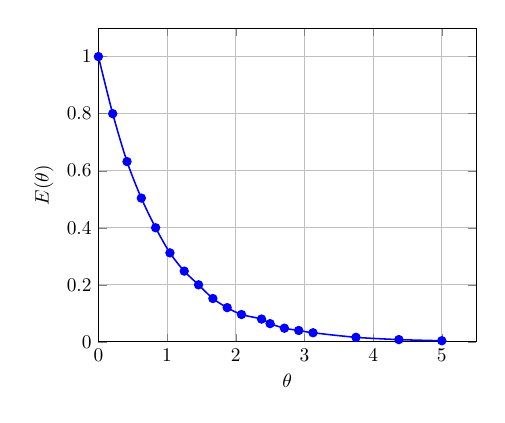
\begin{tikzpicture}[scale=0.7, transform shape]
            \begin{axis}[
                    xlabel={$\theta$},
                    ylabel={$E(\theta)$},
                    ymin=0, ymax=1.1,
                    xmin=0, xmax=5.5,
                    grid=major
                ]
                \addplot[thick, blue,smooth, mark=*] coordinates {
                        (0, 1) (0.2083, 0.8) (0.4167, 0.632) (0.625, 0.504)
                        (0.8333, 0.4) (1.0417, 0.312) (1.25, 0.248) (1.4583, 0.2)
                        (1.6667, 0.152) (1.875, 0.12) (2.0833, 0.096) (2.375, 0.08)
                        (2.5, 0.064) (2.7083, 0.048) (2.9167, 0.04) (3.125, 0.032)
                        (3.75, 0.016) (4.375, 0.008) (5, 0.004)
                    };
            \end{axis}
        \end{tikzpicture}
    \end{minipage}
    \hfill
    \begin{minipage}{0.48\textwidth}
        \centering
        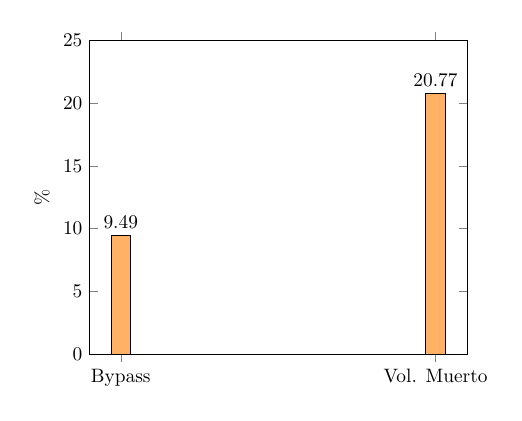
\begin{tikzpicture}[scale=0.7, transform shape]
            \begin{axis}[
                    ybar,
                    symbolic x coords={Bypass, Vol. Muerto},
                    xtick=data,
                    ylabel={\%},
                    ymin=0, ymax=25,
                    nodes near coords
                ]
                \addplot[fill=orange!60] coordinates {(Bypass,9.49) (Vol. Muerto,20.77)};
            \end{axis}
        \end{tikzpicture}
    \end{minipage}
    \caption{Curva de distribución de tiempos de residencia $E(\theta)$ y comportamiento del reactor.}
    \label{fig:comparativa_diagnostico}
\end{figure}
\nt{En la primera subfigura se observa que la curva $E(\theta)$ presenta un perfil característico de un reactor de mezcla completa (CSTR), aunque con un decaimiento más pronunciado.
    Este fenómeno se explica físicamente por la existencia del \textbf{bypass}: al desviarse una fracción del flujo hacia la salida sin pasar por la zona activa, la concentración del trazador en el interior disminuye más rápidamente de lo esperado.
    En la segunda subfigura, el diagnóstico mediante el modelo de compartimentos cuantifica el bypass y el volumen estanco en formato de porcentaje. Matemáticamente, estos valores se obtienen como la diferencia respecto a la unidad ($1 - \text{Integral}$) de los sumatorios resaltados en \textcolor{darkgreen}{verde} en la tabla de cálculo.}
\newpage
\cor{}{
    Volviéndonos a fijar en los sumatorios de las integrales, como en este caso $\int E \,d\theta$ y $\int E\cdot \theta \, d\theta$ son $\neq 1$, entonces sabemos que estamos en el caso de un reactor tanque agitado que debemos modelizar por el modelo mezclado. Simplemente con que una de ellas ya fuera distinta de 1, este sería el modelo a elegir.
}

\begin{table}[htbp]
    \centering
    \begin{tabular}{lc}
        \toprule
        \textbf{Parámetro}                          & \textbf{Valor} \\ \midrule
        Área $\int E \, d\theta$                    & 0.9051         \\
        $\theta_{medio} = \int \theta E \, d\theta$ & 0.7923         \\ \midrule
        \textbf{Resultados:}                        &                \\
        \% Bypass ($1 - \text{Área}$)               & 9.49\%         \\
        \% Vol. Muerto ($1 - \theta_{medio}$)       & 20.77\%        \\ \bottomrule
    \end{tabular}
    \caption{Resultados del diagnóstico hidrodinámico actualizados.}
    \label{tab:diagnostico}
\end{table}

\noindent Como tenemos un volumen estancado del $20.77\%$, es decir, de un tanque total de $800\text{ L}$, $166.16\text{ L}$ corresponderán a un subcompartimento (volumen muerto). Por otro lado, el bypass representa un $9.49\%$, lo que equivale a un caudal desviado de $47.45\text{ L/h}$, tal y como se puede ver en el siguiente esquema.

\begin{center}
    \begin{figure}[htbp]
        \centering
        \begin{tikzpicture}[
            node distance=1cm and 1.5cm,
            reactor/.style={rectangle, draw, thick, minimum width=3cm, minimum height=1.8cm, align=center, fill=white},
            dead/.style={rectangle, draw, thick, minimum width=2cm, minimum height=1.2cm, align=center, fill=gray!10},
            arrow/.style={thick, -{Stealth[scale=1.2]}},
            point/.style={circle, fill, inner sep=1.5pt}
            ]

            % Nodos principales
            \node[reactor] (main) at (2.5,0) {Reactor Activo \\ $V_a = 633.84 \text{ L}$};
            \node[dead, below=0.5cm of main] (deadzone) {Volumen Muerto \\ $V_m = 166.16 \text{ L}$};

            % Entrada
            \node (in) at (-3,0) {};
            \node[point] (split) at (-1,0) {};
            \draw[arrow] (in) -- node[above, pos=0.2] {$F = 500 \text{ L/h}$} (split);

            % Hacia el reactor
            \draw[arrow] (split) -- node[below, blue, pos=0.3] {$F_a = 452.55 \text{ L/h}$} (main.west);

            % Conexión con volumen muerto (intercambio)
            \draw[thick, <->] (main.south) -- (deadzone.north);

            % Salida
            \node[point, fill=red] (merge) at (6,0) {};
            \draw[thick] (main.east) -- node[below] {$X_{AR}$} (merge);
            \node (out) at (8,0) {};
            \draw[arrow] (merge) -- node[above, pos=0.7] {$F = 500 \text{ L/h}$} node[below, pos=1] {$X_{AS}$} (out);

            % Bypass (superior)
            \draw[arrow, rounded corners=10pt] (split) |- (2.5, 1.8) node[above] {Bypass ($v_b = 47.45 \text{ L/h}$)} -| (merge);

        \end{tikzpicture}
        \caption{Modelo de compartimentos: Reactor con flujo real, zona muerta y cortocircuito (Bypass).}
        \label{fig:modelo_compartimentos_rtd}
    \end{figure}
\end{center}
\noindent La forma de resolverlo es aplicando dos balances de materia. Primero en el punto de mezcla (es decir, el marcado en \textcolor{red}{rojo}), aunque previamente es necesario calcular el comportamiento del reactor activo. Los pasos serán los siguientes:

\begin{enumerate}
    \item Como tenemos $V_a$ y $F_a$, podemos calcular $\tau$ para el reactor activo:
          \begin{equation}
              \tau = \frac{V_a}{F_a} = \frac{633.84}{452.55} = 1.40 \si{h^{-1}} \implies \frac{C_{A0}\cdot X_{AR}}{k \cdot C_{A0}\cdot (1-X_{AR})} \implies\frac{\cancel{C_{A0}}\cdot X_{AR}}{1.875 \cdot {\cancel{C_{A0}}\cdot (1-X_{AR})}} \implies X_{AR}= 0.724
          \end{equation}
    \item Realizamos un balance en el punto de mezcla, expresando además la concentración de salida como $C_{AS} = C_{A0}\cdot (1-X_{AS})$ y $C_{AR} = C_{A0}\cdot (1-X_{AR})$:
          \begin{equation}
              F \cdot C_{AS} = F_{\text{bypass}}\cdot C_{A0} + F_a \cdot C_{AR} \implies 500 \cdot  3 \cdot (1-X_{AS}) = 47.45 \cdot 3 + 452.55 \cdot 3 \cdot (1-0.724)
          \end{equation}
\end{enumerate}
\begin{center}
    \Res{X_{AS}= 0.6553 \quad \quad C_{AS} = 1.0341 \text{ M}}
\end{center}
